{\section{Verstärkendes Lernen}}
\label{sec:rl}
Der Begriff 'Verstärkendes Lernen' beschreibt eine Art von Problemstellung und die dafür geeigneten Problemlösungsmethoden im Bereich des Maschinellen Lernens. Die grundlegenden Bestandteile einer Trainingsumgebung sind der Agent und die Umgebung, in der der Agent seine Aktionen ausführt. Der Ansatz ist in vielerlei Hinsicht vergleichbar mit dem Lernvorgang von Menschen. Ein Baby lernt das Krabbeln ohne direkte Anweisungen, nur durch die Wahrnehmung der Umgebung, das Verhalten der Umgebung in Relation zu seinen Bewegungen und die mit den Bewegungen einhergehenden Belohnungen. Auf dieselbe Art lernt der Agent beim Verstärkenden Lernen von jedem Zustand die Aktion auszuführen, um die Belohnung zu maximieren. Die Belohnung können dabei positiv oder negativ sein. Im Fall des Babys sind die Belohnungen Faktoren wie Schmerz, Hunger, Müdigkeit oder gestillte Neugier. Der Agent hingegen erhält eine numerische Belohnung.\cite{sutton2018reinforcement}

\begin{figure}[H]
  \centering  
  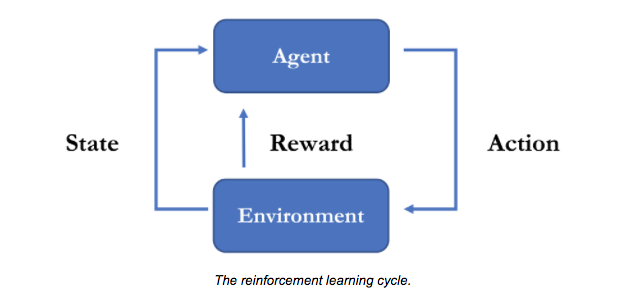
\includegraphics[scale=0.5]{img/rl_cycle.png}
  \caption{Verstärkendes Lernen Ablauf \protect\cite{unity_mlagents_rl_cycle}}
  \label{fig:rl_cycle}
\end{figure}

Die Abbildung 2.1 zeigt die Verbindungen zwischen dem Agent und der Umgebung. Der Agent erhält als Input einen Zustand oder meist einen Teilzustand der Umgebung und reagiert darauf mit einer Aktion. Dieser Zyklus kann je nach Problem in unterschiedlichen Intervallen durchlaufen werden. Bei kontinuierlichen Kontrollproblemen werden Aktionen meist in regelmäßigen Intervallen abgefragt. Bei rundenbasierten Spielen kann dieser Vorgang jedoch auch nur einmal pro Runde stattfinden.